\section{Vorbereitende Aufgaben}
    \subsection{Kürzester Burgers Vektor in LiF}
	Der Burgers - Vektor dient zur Beschreibung eines Gitterbaufehlers. Man erhält ihn, indem man um einen Gitterfehler herum eine (beliebige) geschlossene Kurve aus
	Gittervektoren bildet und dieselbe Kurve im dazugehörigen perfekten Kristall betrachtet. Durch das verschwinden des Gitterfehlers ergibt sich eine Versatzstelle,
	an welcher man den Burgers - Vektor findet (sh. Abb. \ref{FigBurger}).
	
	\begin{figure}[H]
            \centering
            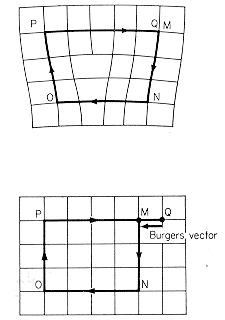
\includegraphics[width=\textwidth]{Images/Burger.gif}
            \label{FigBurger}
            \caption{Konstruktion des Burgers - Vektors. Quelle: https://www.princeton.edu/$\sim$maelabs/mae324/glos324/y58-1.gif}
        \end{figure}

        Da es sich bei LiF um eine FCC-Gitterstruktur handelt, ist der nächste gleichartige Kern stehts an Position $\frac{1}{2} * <110>$. Daraus ergibt sich für den minimalen
        Burgers - Vektor eine Länge von
        \begin{align}
            |<110>| = a \cdot \sqrt{2} \\
            \frac{1}{2} \cdot \frac{a}{\sqrt{2}} = \frac{a}{\sqrt{2}}
        \end{align}
        Längere Burgers - Vektoren sind daher sehr unwahrscheinlich, da die aufzuwendende Energie für eine Verschiebung sich $\propto |\vec{b}|^2$ verhält.


    \subsection{Abstand $d$ zwischen zwei Ätzgrübchen}

	Die Gitterkonstante von LiF beträgt $a = 0.402$nm. Liegen nun zwei Einkristalle in einem sehr kleinen Winkel $\alpha$ zueinander, so können wir aus dem Abstand $d$ der 
	Ätzgrübchen, die durch diese sogenannte Kleinwinkelkorngrenze an der Kristalloberfläche entstehen, genau diesen Winkel bestimmen. Die Formel hierfür erhält man mithilfe
	von $\sin{\alpha} \approx \alpha$ für kleines $\alpha$ wie in Abb. \ref{FigKorn} illustriert:
	\begin{equation}
		\alpha \approx \frac{a}{d} = \frac{0.402nm}{d}
	\end{equation}

	\begin{figure}[H]
            \centering
            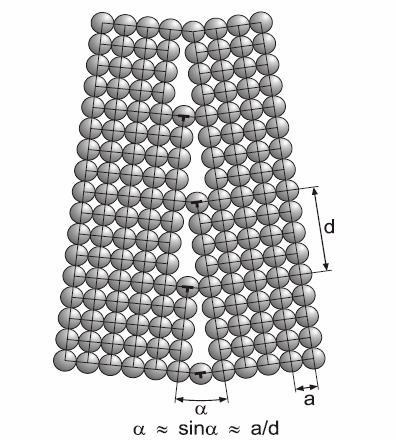
\includegraphics[width=\textwidth]{Images/Korn.JPEG}
            \label{FigKorn}
            \caption{Ätzgrübchenabstand bei Kleinwinkelkorngrenzen. Quelle: https://docplayer.org/docs-images/74/70315204/images/31-0.jpg}
        \end{figure}
 %       \begin{equation}
 %           \theta = \arctan{\frac{b}{d}} = \arctan{\frac{a}{d \sqrt{2}}}
 %       \end{equation}

    \subsection{Versetzungen durch Nadeleindruck}
	\begin{figure}[H]
            \centering
            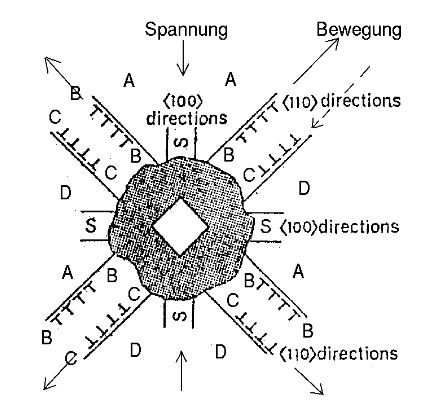
\includegraphics{Images/Question3.PNG}
            \label{FigNadel}
            \caption{Nadeleindruck und aktivierte Gleitsysteme. Quelle: http://muenchuwe.com/nonhtml/papers/fest-25.pdf}
        \end{figure}
	
	Abb. \ref{FigNadel} zeigt die Rosettenform der im Versuch entstehenden Nadeleindrücke sowie die Gittervektoren, entlang derer sich die Strukturen ausbilden. 
	Die im Bild mit S gekennzeichneten Strukturen sind Schraubenversetzungen, die sich entlang der $<100>$ - Richtungen bilden. In $<110>$ - Richtung bilden sich
	Stufenversetzungen, die bei Druck auf die Probe in $\{ \overline{1}00\}$ - Richtung entlang der gekennzeichneten Richtungen wandern. Die Ursache hierfür liegt
	darin, dass bei Druck aus dieser Richtung auf die Probe jeweils die zwei Gleitsysteme von LiF aktiviert werden, die in den ersten zwei Skizzen in Abb. 
	\ref{FigGleitGel} dargestellt sind.
	

	\begin{figure}[H]
            \centering
            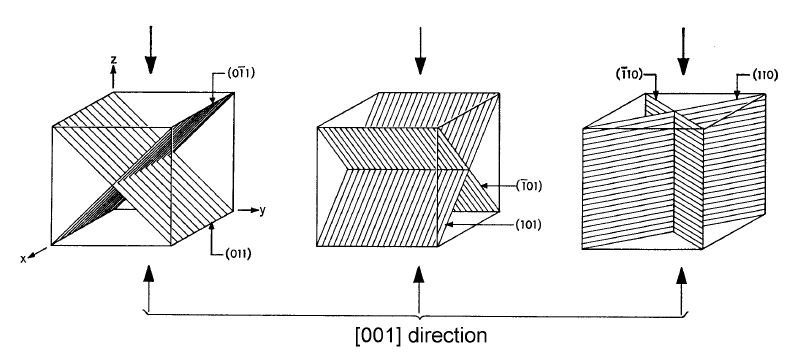
\includegraphics{Images/Gleitsysteme.JPEG}
            \label{FigGleitGel}
            \caption{Gleitsysteme in LiF. Quelle: Praktikumsanleitung}
        \end{figure}

%    \subsection{1234}
%        \hl{Unterschied zwischen Axialem Druck und Nadeleindruck}

	